\chapter{Backend}

\section{Kommunikation}

\subsection{Zeitkritische Informationen}
Als zeitkritisch werden Informationen eingestuft, sofern sie die direkten 
Eingaben der ControlClients und eventuelles Feedback des OutputClient betreffen. 
Da es sich um ein Reaktionsspiel handel,t müssen diese Daten zeitnah von Sender 
zu Empfänger gelangen. Solch eine Relation ist nur über eine Peer-to-Peer 
Verbindung zu realisieren.



\subsection{Möglichkeit 1: Predefined Packages 'rtc.io'}
Der NodeJS Server wird als Verbindungsserver für die Etablierung einer 
Peer-to-Peer Verbindung zwischen ControlClients und OutputClient genutzt. Als 
Technik wird konret WebRTC eingesetzt. Auf dem NodeJS-Server wir das Package 
"rtc-switchboard" eingesetzt, welches eine Grundlage für einen  
Signalisierungsserver ist. Die Clients nutzen "rtc-quickconnect" um neues 
Channels anzufordern und eine Peer-to-Peer Verbindung zu etablieren.

\subsubsection{Vorteile}
\begin{itemize}
\item
Leichtere Implementierung, da alle Ebenen der Kommunikation bereits abgedeckt 
wurden und nur noch semantisch auf Informationen eingegangen werden muss.
\end{itemize}

\subsubsection{Nachteile}
\begin{itemize}
\item
Durch Generalisierung ein deutlicher Overhead.

\item
Status ist offiziell noch 'unstable'.
\end{itemize}



\subsection{Möglichkeit 2: Abstrakte WebRTC implementation 'WebRTC'}
Wie auch bei Möglichkeit 1 wird der NodeJS-Server als Verbindungsserver genutzt. 
Jedoch muss auf Client-Seite, also für OutputClient und ControlClient, eine 
eigene Signalling Implementation stattfinden. Es wird eine viel abtraktere 
Schicht genutzt.

\subsubsection{Vorteile}
\begin{itemize}
\item
Da die genutzen Packages nur eine Grundlage bilden, ist eine spezialisierte 
Implementierung möglich.
\end{itemize}

\subsubsection{Nachteile}
\begin{itemize}
\item
Implementierungsaufwand deutlich höher.

\item
Spezialisierung für dieses Projekt eventuell nicht nötig.

\item
Status ist offiziell noch 'unstable'.
\end{itemize}



\subsection{Möglichkeit 3: Socket.io-P2P}
Das Package Socket.io bietet auch selber eine Peer-to-Peer lösung auf WebRTC 
Basis. Hierbei wird eine Spezielle Art eines Sockets genutzt, welche wie ein 
normaler WebSocket agiert, bis ein Upgrade durchgeführt wird und die Clients nun 
direkt miteinander Kommunizieren.

\subsubsection{Vorteile}
\begin{itemize}
\item
Das Signalling und die P2P Kommunikation können mit einem Package geregelt 
werden.

\item
Variabel kann die Kommunikation über den Server, oder P2P ablaufen.

\item
Signalling events werden von Client-Server Kommunikation direkt zu P2P 
übernommen.
\end{itemize}

\subsubsection{Nachteile}
\begin{itemize}
\item
Wenig Einfluss auf die Upgrade-Mechanismen.
\end{itemize}



\subsection{Möglichkeit 4: Eigenes Kommunikationsmodul}
Aus Basis der WebRTC Standartimplementierung von den Browsern, kann eine eigene Schicht entwickelt werden, welche den Kommunikatinsaufbau (das Signalling) und die Kommunikationsabläufe regelt. Dies müsste auf einer generischen Basis geschehen um allen Anforderungen des Programmes gerecht zu werden.

\subsubsection{Vorteile}
\begin{itemize}
\item
Volle Kontroller über Signalling und Verwaltungsabläufe der Verbindungen.

\item
Möglichkeit für schnelle Anpassungen.

\item
Unabhängigkeit gegenüber anderen Entwicklern.
\end{itemize}

\subsubsection{Nachteile}
\begin{itemize}
\item
Größter Implementierungsaufwand.

\item
Risikoabschätzung nur schwer möglich.

\item
Basis-Implementationen verschieden je Browser (gleiches Problem wie bei den anderen Implementationen: rtc.io, wocket.io-P2P, etc.)
\end{itemize}



\subsection{Statusinformationen}
Für den Austausch von Statusinformationen und Signalen zwischen Peer und Server werden WebSockets genutzt.
Für den Austausch von Statusinformationen zwischen Peers wird WebRTC genutzt.
Für den Austausch von Signalen zwischen Peers werden WebSockets genutzt, wobei der Server der Verbindungs-Knotenpunkt zwischen den Peers ist.



\subsection{Fazit nach Test}
Nach und auch schon während der Entwicklung des Prototypen hat sich 
rausgestellt, dass Socket.io-P2P in der Implementierung viele Fehler aufweist.
Gleiches gilt für rtc.io.
Eine teilweise Abänderung der Module (workarounds) führt näher an das gewünschte Ergebnis, 
verursacht aber intern wieder mehr Fehler und sorgt für eine inkonsistente Modulversion.



\subsection{Fazit}
Die eigene Implementation auf Basis des WebRTC bietet die meisten Möglichkeiten, birgt jedoch auch die meisten Risiken. 
RTC.io bietet eine Implementation die sehr gut für Prototypen geeignet ist, aber neben dem Zeitunkritischen Signalling eine eigene Einheit bietet, welche eine Generalisierung des WebRTC darstellt und somit viel Overhead besitzt. 
Die P2P-Imeplementierung von Socket.io steht von der Implementierungs-Komplexität in der Mitte. Es bietet viele bereits bekannte Mechanismen des Client-Server Signalling über Events, welche mit einem Upgrade nun auch von Client zu Client funktionieren. Dagegen spricht jedoch die instabilität der P2P-Implementation von Socket.io.

Eine eigene Implementation eines Modules auf Basis der von den Browsern gegebenen WebRTC-Schnittstelle ist die Wahl. Sie bietet die größtmögliche Flexibilität im Bezug auf Veränderbarkeit und Anpassung im laufenden Entwicklungszyklus. Als Risiko ist besonders der große Aufwand anzusehen.



\section{Eigenes Modul Kommunikation}
\subsection{Anforderungen an das eigene Modul für WebRTC}
\begin{itemize}
\item 
Es muss möglich sein, unsere ControlPeers nur mit dem DisplayPeer zu verbinden, 
nicht aber untereinander (Sterntopologie, wobei der DisplayPeer das Zentrum ist).

\item
Der DisplayPeer muss zu jedem ihm zugeordneten ControlPeer verbunden sein.

\item
Es Muss auf Serverseite eine Raumlogik existieren, um die Peers zuordnen zu 
können.

\item
Das Signalling muss weiterhin über den Server stattfinden.
\end{itemize}



\subsection{Zuweisungslogik Server}
Der Server hat bezüglich der Zuweisungen für Verbindungen die Aufgabe alle 
Clients zu gruppieren. Dies soll ähnlich wie bei Socket.io über eine Raumlogik 
geschehen. Es existieren Räume, in welche die Sockets auf dem Server (je Client 
also einer) eingeordnet werden.


Hierbei unterscheiden sich die Clients in ihrem Kommunikationsmodus:
\begin{description}
\item[Single]
Ein Client mit dem "Single" Modus pflegt nur eine direkte WebRTC Verbindung.

\item[Multi]
Ein Client mit dem "Multi" Modus pflegt mehrere direkte WebRTC Vebindungen 
gleichzeitig und agiert zwischen den ganzen Peers als "Host".
\end{description}

\begin{figure}[ht]
\centering
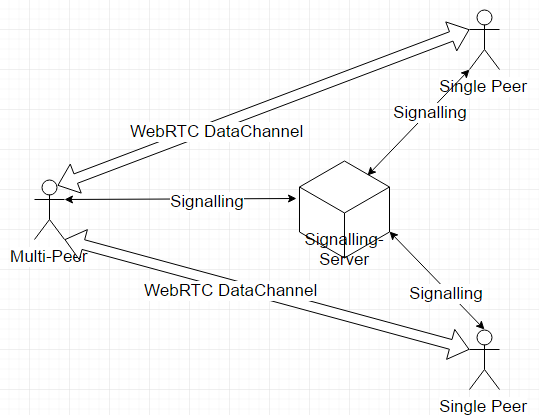
\includegraphics[width=0.9\textwidth]{backend/ConnectionBetweenPeers.PNG}
\caption{Verbindungsnetz}
\label{backfig1}
\end{figure}

In Abbildung \ref{backfig1} ist zu sehen, wie ein "Multi-Peer" mit mehreren 
"Single-Peer" gleichzeitig über WebRTC (konkret den DataChannel) kommuniziert, 
jeder einzelne "Single-Peer" aber nur mit dem einen "Multi-Peer". Zu sehen ist 
außerdem, dass das Signalling weiterhin für alle Peers über den 
Signalling-Server stattfindet, welcher hier auch gleichzeitig der WebServer ist.



\subsection{Zuweisungslogik Client (Single)}
Von nun an wird der Client der den Single Modus nutzt als "Single-Peer" 
bezeichnet.

Der Single-Peer pflegt nur eine WebRTC Verbindung, somit muss keine 
Zuweisungslogik geschehen.



\subsection{Zuweisungslogik Client (Multi)}
Von nun an wird der Client der den Multi Modus nutzt als "Multi-Peer" 
bezeichnet.


Der Multi-Peer pflegt mehrere WebRTC Verbindungen zu verschiedenen Single-Peers. 
Identifiziert werden die einzelnen Single-Peers über ein vom Server beim 
Signalling gesetztes Attribut in den Signalling Nachrichten: "from". Über dieses 
Attribut weiß der Multi-Peer von wem diese Signalling-Message kommt und kann so 
alle ankommenden Informationen diesem Single-Peer zuordnen. Somit wird unter dem 
Alias des Single-Peer ein eigenes "webRTCConnection"-Objekt verwaltet/abgelegt.



\subsection{Identifizierung der Peers}
Die Peers selber erhalten in allen Signalling-Messages ein Attribut, über 
welches sie den Ursprung ermitteln können, um so Signale Peers zuordnen zu 
können. Diese "ID" wird vom Server vergeben und entspricht einfach nur der 
Socket ID welche die einzelnen Clients in Verbindung zum Server haben.
Da nur der Server diese ID vergibt ist diese auch eindeutig.



\section{Signalling Ablauf}
Der Ablauf ist bei den Single-Peers, sowie bei den Multi-Peers nahezu gleich.



\subsection{Anmeldung beim Server}
\begin{description}
\item[Multi-Peer]
Der Multi-Peer meldet sich beim Server mit der Bitte einen Raum zu erstellen. 
Sollte dieser Raum schon existieren ist dies ein Fehler, da in jedem Raum nur 
ein Multi-Peer existieren darf. Sollte der Raum noch nicht existieren, wird er 
erstellt und der Multi-Peer diesem zugewiesen.

\item[Single-Peer]
Der Single-Peer meldet sich beim Server mit der Bitte einen Raum zu betreten. 
Sollte dieser Raum noch nicht existieren ist dies ein Fehler, da ein Raum in 
diesem Projekt ein Spiel darstellt, ein Single-Peer (Control-Peer) aber nur 
einem bestehenden Spiel beitreten kann. Sollte der Raum bereits existieren und 
alle weiteren Spielablaufrelevanten Informationen stimmen (das Spiel darf zum 
Beispiel noch nicht angefangen haben), so tritt der Single-Peer diesem Raum bei. 
Direkt nach dem Beitreten eines Raumes, wird eine Signal an den Server gesendet, 
dass wir da sind.

\item[Server]
Sobald ein Raum existiert und ein Multi-Peer diesem zugewiesen ist, sendet jeder 
neu dazukommende Single-Peer ein Signal an den Server, dass er da ist. Dieses 
Signal wird nur an den Multi-Peer weitergeleitet.
\end{description}



\subsection{Erstes Signal}
\begin{description}
\item[Multi-Peer]
Jedes mal, wenn der Multi-Peer ein neues erstes Signal eines Single-Peers über 
den Server erhält ("hereandready"), ermittelt er seine ICE-Candidates (je nach Browser kann dieses Vorhaben eine erneute Ermittlung der Candidates, oder ein Verwenden der bereits vorher ermittelten veranlassen) und sendet 
diese an den Signalisierenden Single-Peer.
\end{description}



\subsection{ICE Candidates}
\begin{description}
\item[Multi-Peer]
Erhält ein Multi-Peer einen ICE-Candidate wird dieser der Passenden Verbindung 
hinzugefügt und löst das "negotationneeded"-Event aus, welches ein neues Offer 
in Form von SDP Signalisiert.

\item[Single-Peer]
Erhält ein Single-Peer einen ICE-Candidate wird dieser der akutellen 
webRTCCOnnection hinzugefügt und löst das "negotationneeded"-Event, welches ein 
neues Offer in Form von SDP Signalisiert.
\end{description}



\subsection{Aufbau über SDP}
\begin{description}
\item[Multi-Peer]
Erhält der Multi-Peer ein Offer in Form von SDP erwiedert er dieses mit einer 
Answer auch in Form von SDP und fügt die "remoteDescription" dieser 
WebRTCConnection auf Basis der Offer hinzu. Sofern dieser Vorgang Erfolg hatte 
ist eine direkte Verbindung zwischen Multi-Peer und Single-Peer entstanden.

\item[Single-Peer]
Erhält der Multi-Peer ein Offer in Form von SDP erwiedert er dieses mit einer 
Answer auch in Form von SDP und fügt die "remoteDescription" dieser 
WebRTCConnection auf Basis der Offer hinzu. Sofern dieser Vorgang erfolg hatte 
ist eine direkte Verbindung zwischen Multi-Peer und Single-Peer entstanden.
\end{description}



\subsubsection{Kommunikationskanal}
Da es sich um einfache Steuerungsdaten handelt verwenden beide Modi der Peers 
einen simplen DataChannel.



\section{Eigenes Modul: Aufbau}
\subsection{Eigenes Modul: Schnittstelle}
\begin{figure}[ht]
\centering
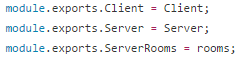
\includegraphics[width=0.9\textwidth]{backend/ModulExports.PNG}
\caption{Modul Exporte}
\label{backfig2}
\end{figure}

\begin{description}
\item[Modul.Client]
Unter Modul.Client ist eine Klassenorientierte Repräsentation des Clients zu 
finden. Es ist ein Object dieses Typs zu erzeugen.

\item[Modul.Server]
Unter Modul.Server ist eine Repräsentation des Servers zu finden. Für jeden auf 
dem Server neu Verbundenen Client muss eine neue (anonyme) Instanz dieses Typs 
erstellt und dabei der Socket der mit dem Client verbunden ist übergeben werden.

\item[Modul.ServerRooms]
Unter Modul.ServerRooms ist eine Simple Liste der derzeitigen Räume auf dem 
Server, inklusive der darin befindlichen Clients zu sehen. Diese Informationen 
sind jedoch nur auf Serverseite bei Verwendung des Modul.Server einsichtlich, 
bzw. werden nur unter Verwendung von Modul.Server aktualisiert.
\end{description}



\subsection{Eigenes Modul: Abhängigkeiten}
Das Modul ist derzeit direkt von Socket.io abhängig, von welchem es die 
WebSockets für das Signalisierungen über den Signalling-Server nutzt.



\subsection{Eigenes Modul: Struktur}
Das Modul implementiert zwei Teile. Erstens die Client-Seite. Zweitens die 
Server-Seite.



\subsubsection{Client Aufgaben}
Die Client-Implementation ist für das Frontend gedacht und nutzt alle WebRTC 
Standarts der Browserimplementationen (Mozilla, webkit und Microsoft überlagert). 
Es handelt alle Faktoren von Initiierung der Kommunikation, bis Durchführung dieser ab.



\subsubsection{Server}
Die Server-Implementation kümmert sich auf Server-Seite um die Einhaltung von 
Kommunikations-Standarts, die Zuweisung von Signalen und die Gruppierung vieler 
Peers.



\section{Eigenes Modul: Generischer Ansatz}

\subsection{Generische Anforderung}
Als Anfoforderung gilt, dass die Implementierung des Moduls von unserer Nutzung für das Ping-Pong Projekt entkoppelt ist. Dies ist als gegeben anzusehen, wenn die Implementation keine Hinweise auf dieses Projekt hinterlässt und Möglichkeiten zu Umsetzung anderer beliebiger Projekte bietet, ohne Anpassungen vornehmen zu müssen.



\subsection{Generische Umsetzung}
Im folgenden wird die allgemeine generische Umsetzung am Beispiel der Callbacks und Topologien gezeigt.

\subsubsection{Generische Umsetzung: Allgemein}
Im allgemeinen gibt es zwei Klassen von Peers, die ein Client nutzen kann.
\begin{description}
\item[Single-Peer]
Ein Client der den Modus "Single-Peer" nutzt gibt damit an, dass er maximal eine direkte Verbindung zu einem anderen Peer pflegen möchte.

\item[Multi-Peer]
Ein Client der den Modus "Multi-Peer" nutzt gibt damit an, dass er eine oder mehr direkte Verbindungen zu Peers pflegen möchte.
\end{description}

Aus Kombinationen dieser Modi lassen sich verschiedene Topologien bilden. Näheres unter "Generische Umsetzung: Topologien".



\subsubsection{Generische Umsetzung: Callbacks}
Um jeden Nutzer dieses Moduls selbst die Verarbeitung von Ereignissen zu ermöglichen, ist die Möglichkeit gegeben, dass der Nutzer Callback-Funktionen hinterlegt, die bei gewissen autretenden Ereignissen ausgerufen werden.
Diese Ereignisse umfassen z.B:
\begin{description}
\item[Neue Verbindung]
Eine neue Verbindung zu einem Peer wurde erfolgreich hergestellt.

\item[Verbindungsverlust zu Peer]
Eine bestehende Verbindung zu einem Peer wurde verloren.

\item[Neue Nachricht]
Es kam eine neue Nachricht über den DataChannel eines Peers an.
\end{description}

Weiteres zu der direkten Verwendung der Callback-Functionen unter "Eigenes Modul Verwendung: Callbacks".



\subsubsection{Generische Umsetzung: Topologien}
Es lassen sich durch die Verwendung der zwei Modi verschiedene Topologien bilden.
\begin{description}
\item[one-to-one]
Keine konkrete Topologie, aber für direkte Peer-to-Peer Verbindungen oft die gängiste Art. Beide Peers sind "Single-Peer" und pflegen jeweils nur die Verbindung zu dem anderen. 
Siehe Abbildung \ref{backfig3}.
\begin{figure}[ht]
\centering
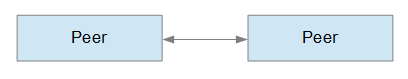
\includegraphics[width=0.9\textwidth]{backend/Topologie_1v1.PNG}
\caption{Topologie one-to-one}
\label{backfig3}
\end{figure}

\item[Stern]
Einer der Peers agiert als Host für die anderen. Dieser Host-Peer ist der Mittelpunkt des Sternes und nutzt den Modus "Multi-Peer". Alle anderen Peers nutzen den Modus "Single-Peer" und pflegen nur die Verbindung zum Mittelpunkt (dem Host).
Siehe Abbildung \ref{backfig4}.
\begin{figure}[ht]
\centering
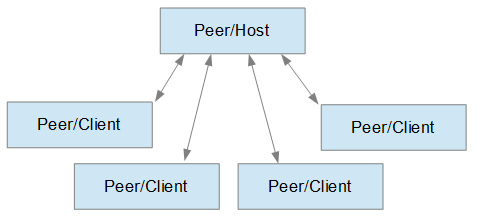
\includegraphics[width=0.9\textwidth]{backend/Topologie_4v1.PNG}
\caption{Topologie Stern}
\label{backfig4}
\end{figure}

\item[Vollvermascht]
Alle Peers nutzen den Modus "Multi-Peer" und pflegen zu jedem anderen Peer eine direkte Verbindung.
Siehe Abbildung \ref{backfig5}.
\begin{figure}[ht]
\centering
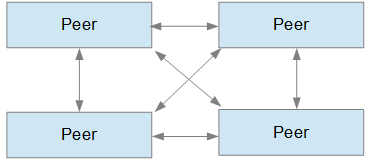
\includegraphics[width=0.9\textwidth]{backend/Topologie_ava.PNG}
\caption{Topologie Vollvermascht}
\label{backfig5}
\end{figure}

\end{description}


\section{Eigenes Modul: Verwendung}

\subsection{Eigenes Modul Verwendung: Client}
\subsection{Eigenes Modul Verwendung: Server}
\begin{figure}[ht]
\centering
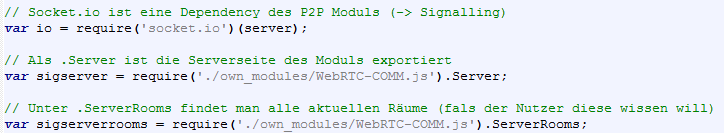
\includegraphics[width=0.9\textwidth]{backend/Modul_UserServerDependencies.PNG}
\caption{Dependencies Verwendung Server}
\label{backfig6}
\end{figure}
In Abbildung \ref{backfig6} ist zu sehen, welche Abhängigkeiten auf Serverseite bestehen.
Für das Signalling nutzt das Modul die Serverseitige Implementation von "socket.io". 
Zur Nutzung des Moduls muss dieses außerdem "required" werden. Hierzu wird der Pfad zu dem Modus als Parameter an das require übergeben und der Server Export genutzt.
Die Verwendung der ServerRooms ist optional und gibt dem Nutzer die Möglichkeit auf dem Server eine Einsicht in die derzeitigen Räume zu erlangen und über WebSockets die in diesen hinterlegt sind mit den Clients zu Kommunizieren.

\begin{figure}[ht]
\centering
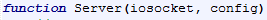
\includegraphics[width=0.9\textwidth]{backend/Modul_ServerContructor.PNG}
\caption{Server Konstruktor}
\label{backfig7}
\end{figure}
In Abbildung \ref{backfig7} ist der allgemeine Konstruktor des Moduls für Server zu sehen.

\begin{figure}[ht]
\centering
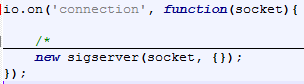
\includegraphics[width=0.9\textwidth]{backend/Modul_UserServerHowTo.PNG}
\caption{Nutzung Server}
\label{backfig8}
\end{figure}
In Abbildung \ref{backfig8} ist zu sehen, wie das Modul für Server genutzt wird. Für jeden neuen Client der sich erfolgreich mit dem Server verbunden hat muss ein neues Modul.Server Objekt erstellt werden. An dieses Modul muss der Socket (socket.io) und etwaige optionale Parameter/Optionen übergeben werden. Die Erstellung dieses Objektes führt dazu, dass Eventhandler des WebSocket für das Handling des Signalling erstellt werden und der Nutzer einem Raum zugewisen werden kann. Dies geschieht alles automatisch und intern im Modul. Der in Abbildung \ref{backfig8} zu sehende Code stellt die Minimalimplementation dar, wie sie auch im Projekt "Ping-Pong" verwendet wird. In den meisten Fällen reicht diese aus.



\subsection{Eigenes Modul Verwendung: Callbacks}



\section{Eigenes Modul: Performance}

\subsection{Eigenes Modul Performance: Beispiel am Projekt}
\subsection{Eigenes Modul Performance: Beispiel für Chat}
\subsection{Eigenes Modul Performance: Beispiel extreme}



\section{Eigenes Modul: Möglichkeiten}

\subsection{Eigenes Modul Möglichkeiten: Verwendbar}
\subsection{Eigenes Modul Möglichkeiten: Erweiterbar}